\chapter{Conclusion}
brief of conclusion

\section{Jesron Marudut Hatuan /1164077}
\subsection{Teori}
\begin{enumerate}
\item Alasan mengapa Kata-Kata harus dilakukan vektorisasi lengkapi dengan ilustrasi gambar.
\subitem Kata kata harus dilakukan vektorisasi dikarenakan untuk mengukur nilai kemunculan suatu kata yang sama dari sebuah kalimat sehingga kata-kata tersebut dapat di prediksi berapa kemunculanya. Atau juga di buatkan vektorisasi data yang digunakan untuk memprediksi bobot dari suatu kata misalkan mobil dan motor sama-sama kendaraan maka akan dibuat prediksi apakah kata tersebut akan muncul pada kalimat yang kira-kira memiliki bobot yang sama. 
\par Untuk ilustrasinya dapat dilihat pada gambar \ref{c5_1}
\begin{figure}[ht]
\centerline{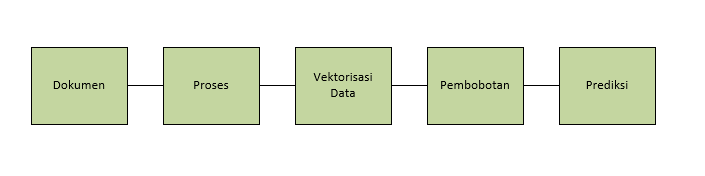
\includegraphics[width=1\textwidth]{figures/c5t/1.png}}
\caption{Ilustrasi Soal No. 1}
\label{c5_1}
\end{figure}
\item Alasan Mengapa dimensi dari vektor dataset google bisa mencapai 300 lengkapi dengan ilustrasi gambar.
\subitem Dimensi dari vektor dataset google bisa mencapai 300 karena dimensi dari vektor digunakan untuk membandingkan bobot dari setiap kata, misalkan terdapat kata mobil dan motor pada dataset google tersebut setiap kata tersebut di buat dimensi vektor 300 untuk kata mobil dan 300 dimensi vektor juga untuk kata motor kemudian kata tersebut di bandingkan bobot kesamaan katanya maka akan muncul akurasi sekitar 70an persen kesamaan bobot dikarenakan kata mobil dan motor sama sama di gunakan sebagai kendaraan.
\par Untuk ilustrasinya dapat dilihat pada gambar \ref{c5_2}
\begin{figure}[ht]
\centerline{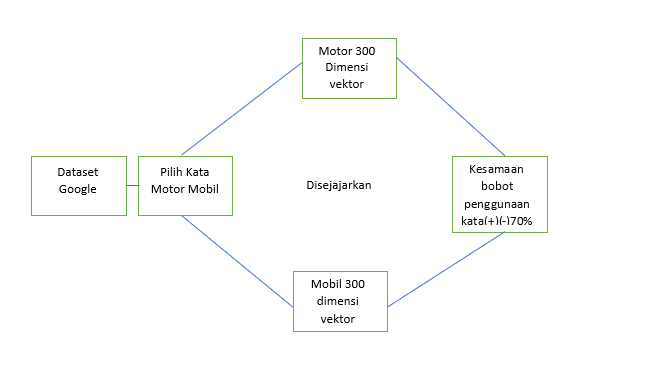
\includegraphics[width=1\textwidth]{figures/c5t/2.png}}
\caption{Ilustrasi Soal No. 2}
\label{c5_2}
\end{figure}
\item Penjelasan tentang konsep vektorisasi untuk kata dan dilengkapi dengan ilustrasi atau gambar.
\subitem Konesp vektorisasi untuk kata yaitu mengetahui kata tengah dari suatu kalimat utama dengan suatu kalimat contoh ( Jangan lupa like dan comment yah makasih ) kata tengah tersebut merupakan (dan) yang memiliki bobot sebagai kata tengah dari suatu kalimat atau bobot sebagai objek dari suatu kalimat. hal ini sangat berkaitan dengan dimensi vektor pada dataset google yang 300 tadi karena untuk mendapatkan nilai atau bobot dari kata tengah tersebut di dapatkan dari proses dimensiasi dari kata tersebut. 
\par Untuk ilustrasinya dapat dilihat pada gambar \ref{c5_3}
\begin{figure}[ht]
\centerline{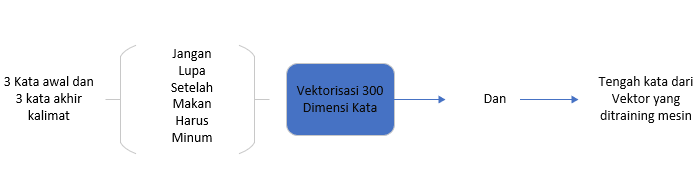
\includegraphics[width=1\textwidth]{figures/c5t/3.png}}
\caption{Ilustrasi Soal No. 3}
\label{c5_3}
\end{figure}
\item Penjelasan konsep vektorisasi untuk dokumen dan dilengkapi dengan ilustrasi atau gambar.
\subitem Konsep vektorisasi untuk dokumen hampir sama seperti vektorisasi untuk kata hanya saja pemilihan kata utama atau kata tengah terdapat pada satu dokumen jadi mesin akan membuat dimensi vektor 300 untuk dokumen dan nanti kata tengahnya akan di sandingkan pada dokumen yang terdapat pada dokumen tersebut.
\par Untuk ilustrasinya dapat dilihat pada gambar \ref{c5_4}
\begin{figure}[ht]
\centerline{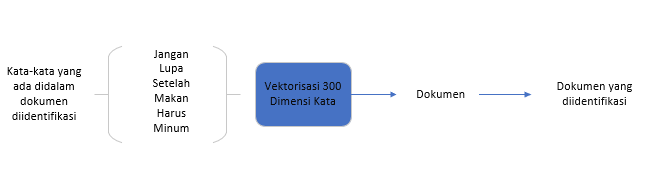
\includegraphics[width=1\textwidth]{figures/c5t/4.png}}
\caption{Ilustrasi Soal No. 4}
\label{c5_4}
\end{figure}
\item Penjelasan dari mean dan standar deviasi,beserta ilustrasi atau gambar.
\subitem Mean adalah nilai rata-rata dari suatu data. Mean disini merupakan petunjuk terhadap kata-kata yang di olah jika kata kata itu akurasinya tinggi berarti kata tersebut sering muncul begitu juga sebaliknya. Standar deviasi merupakan standar untuk menimbang kesalahan.
\par Untuk ilustrasinya dapat dilihat pada gambar \ref{c5_5}
\begin{figure}[ht]
\centerline{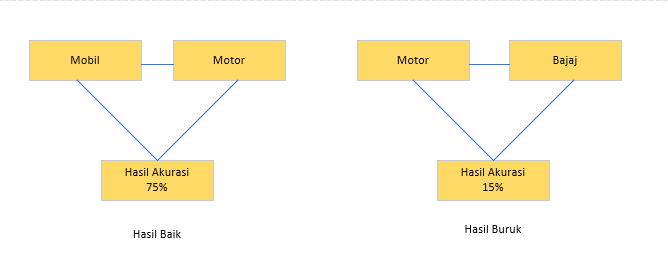
\includegraphics[width=1\textwidth]{figures/c5t/5.png}}
\caption{Ilustrasi Soal No. 5}
\label{c5_5}
\end{figure}
\item Penjelasan Skip-Gram beserta contoh ilustrasi.
\subitem Skip-Gram yaitu dimana kata tengah menjadi acuan terhadap kata kata pelengkap dalam suatu kalimat.
\par Untuk ilustrasinya dapat dilihat pada gambar \ref{c5_6}
\begin{figure}[ht]
\centerline{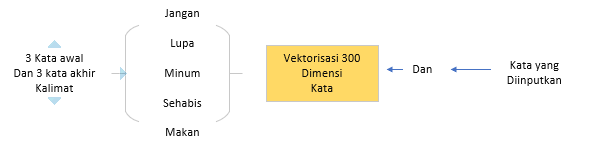
\includegraphics[width=1\textwidth]{figures/c5t/6.png}}
\caption{Ilustrasi Soal No. 6}
\label{c5_6}
\end{figure}
\end{enumerate}

\subsection{Praktek Program}

\section{Conclusion of Problems}
Tell about solving the problem

\section{Conclusion of Method}
Tell about solving using method

\section{Conclusion of Experiment}
Tell about solving in the experiment

\section{Conclusion of Result}
tell about result for purpose of this research.
